% Copyright 2022 Edoardo Riggio

% Licensed under the Apache License, Version 2.0 (the "License");
% you may not use this file except in compliance with the License.
% You may obtain a copy of the License at

% 	http://www.apache.org/licenses/LICENSE-2.0

% Unless required by applicable law or agreed to in writing, software
% distributed under the License is distributed on an "AS IS" BASIS,
% WITHOUT WARRANTIES OR CONDITIONS OF ANY KIND, either express or implied.
% See the License for the specific language governing permissions and
% limitations under the License.

\documentclass{article}

\usepackage{hyperref, amsmath, graphicx, amssymb, csquotes, tabularx}
\usepackage{fancyvrb,newverbs,xcolor}

\graphicspath{ {./assets/} }

\definecolor{cverbbg}{gray}{0.93}

\newenvironment{cverbatim}
 {\SaveVerbatim{cverb}}
 {\endSaveVerbatim
  \flushleft\fboxrule=0pt\fboxsep=.5em
  \colorbox{cverbbg}{\BUseVerbatim{cverb}}%
  \endflushleft
}

\newenvironment{lcverbatim}
 {\SaveVerbatim{cverb}}
 {\endSaveVerbatim
  \flushleft\fboxrule=0pt\fboxsep=.5em
  \colorbox{cverbbg}{%
    \makebox[\dimexpr\linewidth-2\fboxsep][l]{\BUseVerbatim{cverb}}%
  }
  \endflushleft
}

\def\changemargin#1#2{\list{}{\rightmargin#2\leftmargin#1}\item[]}
\let\endchangemargin=\endlist 

\newcommand{\ctexttt}[1]{\colorbox{cverbbg}{\texttt{#1}}}
\newverbcommand{\cverb}
  {\setbox\verbbox\hbox\bgroup}
  {\egroup\colorbox{cverbbg}{\box\verbbox}}

\begin{document}
\begin{titlepage}
    \begin{center}
        \vspace*{1cm}
        
        \Huge
        \textbf{Distributed Systems Cheatsheet}
        
        \vspace{0.5cm}
        \LARGE
        
        \vspace{.5cm}
        
        Edoardo Riggio
   		  \vspace{1.5cm}
       
        \vfill
        
        \today
        
        \vspace{.8cm}
          \Large
          Distributed Systems - S.A. 2022 \\
        Software and Data Engineering \\
        Universit\`{a} della Svizzera Italiana, Lugano \\
        
    \end{center}
\end{titlepage}

\tableofcontents

\newpage

\section{Introduction}
With the advent in the mid 1980's of 16-, 32-, and 64-bit CPUs -- as well as the invention of high-speed computer networks, made it possible for the creation of large numbers of geographically-dispersed networks of computers. These are known as \textbf{distributed systems}.

\subsection{Definition}
A distributed system is a collection of independent computers that appear to the user as a single coherent system. \\ \\
Each computing element of these massive systems are able to behave independently from one another. A computing element is often referred to as a \textbf{node}. This node can either be a hardware device or a software process.

\subsection{Consequences}
Some of the main negative consequences that arise when dealing with distributed systems are the following:

\begin{itemize}
	\item \textbf{Concurrency} \\
	This happens when several processes try to read and write on a shared storage service.
	
	\item \textbf{Absence of a global clock} \\
	Each node will have its own notion of time. This means that there is no common reference of time between the nodes.
	
	\item \textbf{Failure independency}
	The failure of a node can make another node unusable.
	
\end{itemize}

\subsection{Challenges}
Some of the challenges that arise when dealing with distributed systems are outlined in the following sections.

\subsubsection{Openness}
The services are offered according to standard rules. These rules describe both the syntax and semantics of such services. The standard rules of distributed systems are called \textbf{COBRA}(Common Object Request Broker Architecture).

\subsubsection{Scalability}
Scalability can be with respect to the \textbf{system size} -- which would mean adding more users to the system; to the \textbf{geography} -- which would deal with users lying far apart from one another; and to \textbf{administration} -- which would deal with the complexity to manage an increasing system. \\ \\
Some scalability techniques are the following:

\begin{itemize}
	\item \textbf{Hiding communication latencies} \\
	This is important for \textbf{geographical scalability}. Asynchronous communications can be used to reduce the waiting time of the users. This can be achieved with the use of batch processing and parallel applications.
	
	\item \textbf{Distribution} \\
	Components are split into parts and spread across the system. An example of this would be the DNS, where we have a tree of domains divided into non-overlapping zones. Furthermore, the name in a zone is handled by a single name service.
	
	\item \textbf{Replication} \\
	This can be use to increase both \textbf{availability} and \textbf{performance}, as well as reduce \textbf{latency}. Moreover, caching can be used as a form of replication, but is typically done on-demand.
\end{itemize}

\subsubsection{Transparency}
Transparency is the ability of a system to hide some of its characteristics or errors to the user. There exist several different forms of transparency:

\begin{itemize}
	\item \textbf{Access transparency} \\
	Hide the differences in data representation and machine architecture.
	
	\item \textbf{Location transparency} \\
	Users cannot tell where a resource is physically located.
	
	\item \textbf{Relocation transparency} \\
	Even if the entire service was moved from one data center to the other, the user wouldn't be able to tell.
	
	\item \textbf{Migration transparency} \\
	Moving processes and resources initiated by users, without affecting any ongoing communication and operation.
	
	\item \textbf{Replication transparency} \\
	Hide the existence of multiple replicas of one resource.
	
	\item \textbf{Concurrency transparency} \\
	Each user is not going to notice if another user is making use of the same resource.
	
	\item \textbf{Failure transparency} \\
	The user or application does not notice that some piece of the system fails to work properly. The system is then able to automatically recover from the failure.
\end{itemize}

\subsection{Types of Distributed Systems}
There are three main types of distributed systems: \textbf{distributed computing systems}, \textbf{distributed information systems}, and \textbf{distributed pervasive systems}.

\subsubsection{Distributed Computing Systems}
These systems aim at high-performance computing tasks. These systems can be part of two subtypes:

\begin{itemize}
	\item \textbf{Cluster Computing} \\
	All the resourced are located in a local-area network, and are using the same OS. In addition, they also have a common administrative domain.
	
	\item \textbf{Grid Computing} \\
	This is a "federation" of computer systems. Such systems may have different administrative domains, different hardware, software... Such systems are used to make collaboration between organisations feasible.
\end{itemize}

\subsubsection{Distributed Information Systems}
These systems are based on transactions. These transactions are used to make systems communicate between themselves. Transactions follow the \textbf{ACID} properties:

\begin{itemize}
	\item \textbf{Availability} \\
	To the user, the transaction happens indivisibly.
	
	\item \textbf{Consistency} \\
	The transaction does not violate system invariants.
	
	\item \textbf{Isolation} \\
	Concurrent transactions do not interfere with each other.
	
	\item \textbf{Durability} \\
	Once a transaction commits, the changes are permanent.
\end{itemize}

\noindent The application components of each node communicate directly with each other.

\subsubsection{Distributed Pervasive Systems}
These systems are composed by mobile and embedded computing devices. This means that pervasive systems need to have the following characteristics:

\begin{itemize}
	\item Embrace contextual changes
	\item Encourage ad-hoc composition
	\item Recognise sharing as the default
\end{itemize}

\noindent Some examples of such architectures are home systems, electronic health care systems, and sensor networks.

\section{Architectures}
In a distributed system there are two types of architectures:

\begin{itemize}
	\item \textbf{Software Architectures} \\
	How software components are organised and interact between each other.
	
	\item \textbf{System Architectures} \\
	How software components are instantiated on real machines.
\end{itemize}

\subsection{Software Architectures}
Software architectures are based on \textbf{components}, which are modular units with well-defined interfaces. Software architectures can be of several different types:

\begin{itemize}
	\item \textbf{Layered architectures}
	\item \textbf{Object-based architectures}
	\item \textbf{Data-centred architectures}
	\item \textbf{Event-based architectures}
\end{itemize}

\subsubsection{Layered Architectures}
In this kind of architecture, the components at layer $L_i$ can call components in layer $L_{i-1}$, but not components in layer $L_{i+1}$.

\begin{center}
	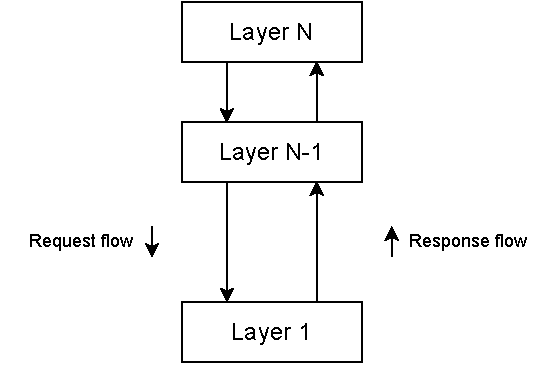
\includegraphics[width=7cm, height=5cm, keepaspectratio]{assets/layered.pdf}
\end{center}

\subsubsection{Object-Based Architectures}
Each object is a component connected through a remote procedure call mechanism.

\begin{center}
	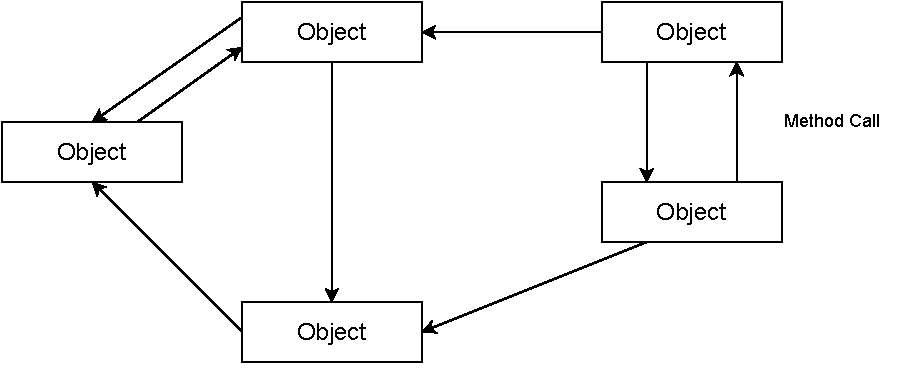
\includegraphics[width=11cm, height=5cm, keepaspectratio]{assets/object-based.pdf}
\end{center}

\subsubsection{Data-Centred Architectures}
The processes communicate through a common repository. This repository can be, for example, a shared distributed file system or a database.

\begin{center}
	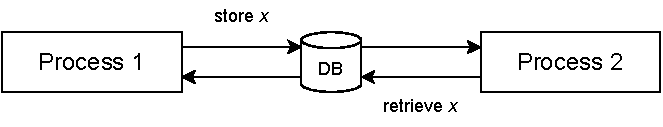
\includegraphics[width=8cm, height=5cm, keepaspectratio]{assets/data-centered.pdf}
\end{center}

\subsubsection{Event-Based Architectures}
The processes communicate through the propagation of events (\textbf{publish-subscribe system}). The middleware ensures that the process which subscribes to that events will receive them. \\ \\
Processes are loosely coupled, this means that they do not to refer to each other.

\begin{center}
	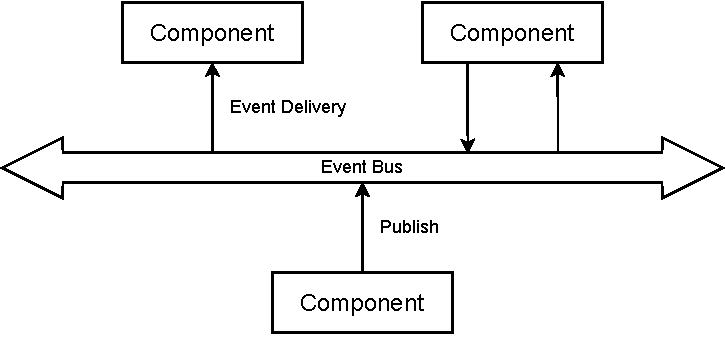
\includegraphics[width=9cm, height=5cm, keepaspectratio]{assets/event-based.pdf}
\end{center}

\subsubsection{Shared Data-Space Architecture}
These architectures are similar to data-centred and event-based architectures.

\begin{center}
	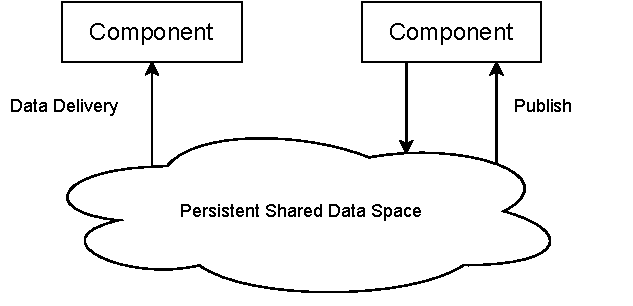
\includegraphics[width=8cm, height=5cm, keepaspectratio]{assets/shared.pdf}
\end{center}

\subsection{System Architectures}
System Architectures describe what software components are used, where to place each component, and how the components interact with each other. \\ \\
There are two types of system architectures:

\begin{itemize}
	\item \textbf{Centralised architectures}
	\item \textbf{Decentralised architectures}
\end{itemize}

\subsection{Centralised Architecture}
Centralised architectures follow the Client-Server model. The \textbf{server} implements some services, while the \textbf{client} requests services and waits for replies. \\ \\
The communication between server and client is \textbf{connectionless}. This means that it is highly efficient, but it is more complex to handle transmission failures (UDP). \\ \\
Server and client may also use another way to communicate. This protocol is connection-oriented, relatively low performance, but more reliable. This is because the node makes a request and receives a reply back in the same connection. \\ \\
Centralised architectures can be either \textbf{single-} or \textbf{multi-layered}. Multi-layered architectures enable to divide concerns, meaning that clients can contain only the program implementing the user-interface level (or only part of it). Moreover, architectures can also be \textbf{multi-tiered}.

\subsection{Decentralised Architectures}
Decentralised architectures can be either vertically or horizontally distributed.

\begin{itemize}
	\item \textbf{Vertical Distribution} \\
	It can be achieved by placing logically different components on different machines. An example of this is a three-tiered application.
	
	\item \textbf{Horizontal Distribution} \\
	Both clients and servers are physically split up into logically equivalent parts. Each part operates on its own share of the dataset. An example of this is a peer-to-peer system.
\end{itemize}

\subsubsection{Structured Peer-to-Peer Architectures}
Structured peer-to-peer architectures are deterministic procedures used to build an \textbf{overlay network}. Here nodes are processes, and links are possible communication channels. \\ \\
In the case of a structured peer-to-peer architecture, we use \textbf{Distributed Hash Tables} (DHT). Each data item that is maintained by the system, is uniquely associated with a key, and this key is subsequently used as an index. Moreover, to each node of the system is assigned an identifier. Each node is made responsible for storing data associated with a specific subset of keys. \\ \\
Any node can be asked to look up a given key, which boils down to efficiently routing that lookup request to the node responsible for storing the data associated with the given key. \\ \\
An example of a structural peer-to-peer architecture is a \textbf{Chord}, which is depicted below.

\begin{center}
	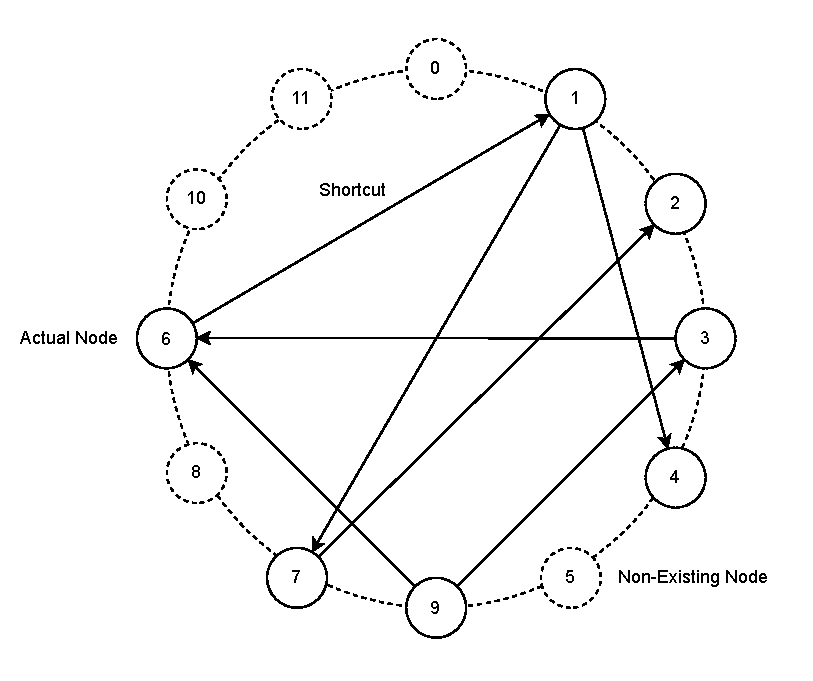
\includegraphics[width=12cm, height=9.5cm, keepaspectratio]{assets/chord.pdf}
\end{center}

\subsubsection{Unstructured Peer-to-Peer Architectures}
In this type of architecture, the overlay network is built using a randomised procedure. Each node in the network has a list of neighbours, constructed in a random way. This results in a random graph. \\ \\
In these kinds of systems, when a node joins the network, it often contacts a well-known node to obtain a starting list of other peers in the system. Moreover, the nodes generally change their local list almost continuously. \\ \\
Unlike in structured peer-to-peer architectures, looking up data cannot follow a predetermined route. Instead, in this case we need to resort to searching for data. This can be done in different ways, such as \textbf{flooding}, \textbf{random walks}, or \textbf{policy-based} search methods.

\begin{center}
	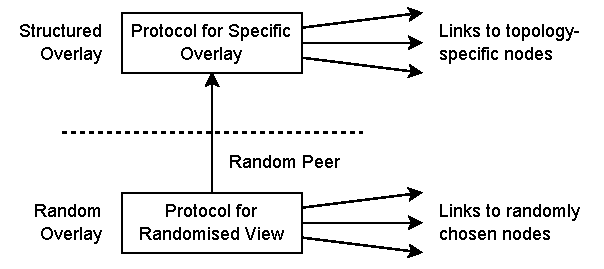
\includegraphics[width=8cm, height=5cm, keepaspectratio]{assets/unstructured.pdf}
\end{center}

\subsection{Super Peer}
\textbf{Brokers} are services that collect data on resource usage and availability for a number of nodes that are in each other's proximity. This allows to quickly select the node with sufficient resources. \\ \\
Nodes that act as brokers are called \textbf{super peers}. Super peers organise themselves into a structured peer-to-peer network, leading to a hierarchical organisation of nodes. The nodes that connect to these super peers are known as \textbf{weak peers}.

\begin{center}
	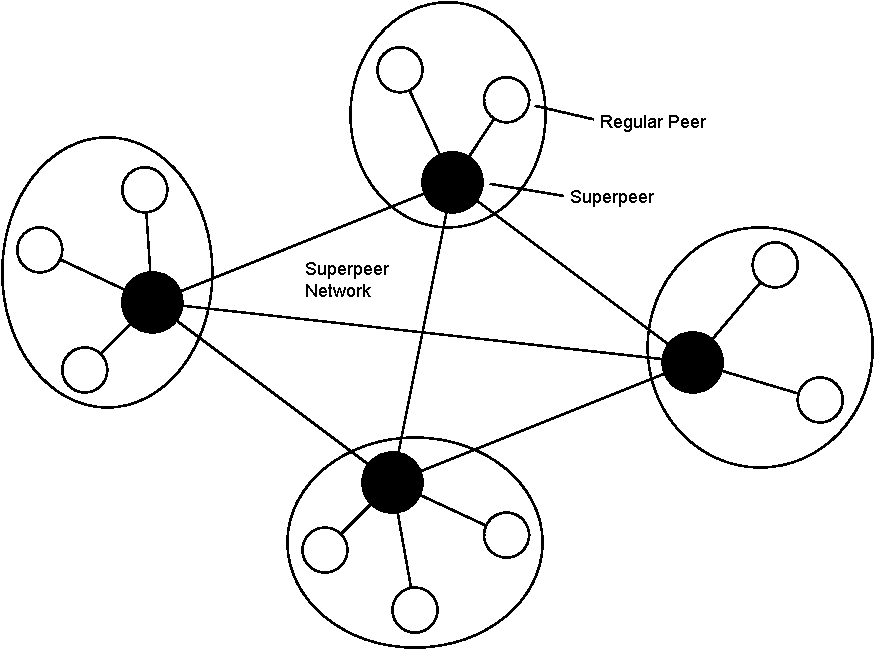
\includegraphics[width=9cm, height=10cm, keepaspectratio]{assets/superpeer.pdf}
\end{center}

\subsection{Middleware}
Middleware provides a degree of distribution transparency. They can either follow an object-based architectural style, or an event-based architectural style.

\subsubsection{Interceptors}
They offer a means to adapt the middleware. Interceptors break the usual flow of control and allow other application-specific code to be executed. Moreover, they are used to improve software management.

\subsubsection{Wrappers and Adapters}
Wrappers and adapters provide a similar interface to the original abstraction, and implement additional logic before or after invoking the original interface.

\subsubsection{Proxies and Stubs}
They provide -- as in the case of wrappers and adapters -- a similar interface as the original abstraction. However, in this case proxies and stubs usually own components rather than extending previously defined ones.

\section{Processes}
\subsection{Introduction}
Virtual processors are created by the OS. A process is a program executed on one of these virtual processors. Each processor has a process table in which several different values relative to the process are stored. \\ \\
Concurrent processes are protected from each other by making the sharing of CPU and hardware resources transparent and using special hardware. \\ \\
Every time a new process is created, the OS must create an independent address space as well. This is known as \textbf{context switching}, and it's really expensive.

\subsection{Threads}
A thread is a lightweight process that can run inside of a process. Threads share the same memory space. For this reason, context switching between threads is less expensive than between processes. \\ \\
Threads are used in distributed systems mainly for making communication calls non blocking. \\ \\
In the case of servers with \textbf{single-threaded models}, one thread receives the request and executes it rapidly. This is known as sequential processing. \\ \\
On the other hand, in the case of servers with \textbf{finite state machine models}, one thread executes the requests and the replies. Blocking system calls are replaced by non-blocking ones, and multiple requests can be handled in parallel.

\subsection{Virtualisation}
The role of virtualisation -- in distributed systems -- is to extend or replace existing interfaces and mimic the behaviour of other systems. \\ \\
The main reasons of virtualisation are the following:

\begin{itemize}
	\item Allow legacy software to run on new mainframe hardware
	\item Porting legacy interfaces to new platforms
	\item Isolating systems running on the same server
\end{itemize}

\subsection{Superservers}
A superserver is a kind of server that listens on many ports and fork a process to execute a service.

\subsection{Stateless vs Stateful Servers}
A server is said to be \textbf{stateless} if it does not keep any information about the state of the client. \\ \\
On the other hand, a server is said to be \textbf{stateful} if it maintains persistent information about the clients. This solution is better in terms of performance (it caches data of the users), but can be problematic in the case that the server crashes or experience other memory-related issues.

\subsection{Server Clusters}
A server cluster is a collection of machines connected through a network. Such clusters have three tiers:

\begin{enumerate}
	\item \textbf{Logical Switch} \\
	It receives client requests and route them to the servers.
	
	\item \textbf{Application Servers} \\
	Low-end servers are used when the storage is the bottleneck of the system. Otherwise, high-end servers are used when the service deals with computationally expensive computations.
	
	\item \textbf{Data-Processing Servers} \\
	The databases.
\end{enumerate}

\section{Communication}
In layered protocols, process \textit{A} con communicate with process \textit{B} by building a message in its address space. After doing so, a system call is used to send the message from \textit{A} to \textit{B}.

\subsection{OSI Model}
The \textbf{Open System Interconnection} (OSI) \textbf{Reference Model} is an ISO standard. This type of model is never widely used or implemented. \\ \\
The OSI model makes use of connection-oriented protocols. Both the sender and the receiver explicitly establish a connection, they communicate, and finally explicitly terminate the connection. \\ \\
The OSI model is divided into the following parts:

\begin{itemize}
	\item Application layer
	\item Presentation layer
	\item Session layer
	\item Transport layer
	\item Network layer
	\item Data link layer
	\item Physical layer
\end{itemize}

\noindent In the following sections, we will have a bottom-up look at the different layers.

\subsubsection{Physical Layer}
This layer deals with how to send bits from one end to the other. It standardises electrical, mechanical, and signalling interfaces. finally, it does not handle errors.

\subsubsection{Data Link Layer}
The data link layer groups the bits into frames and ensures their correct transmission. It uses checksums to verify the integrity of the data frames.

\subsubsection{Network Layer}
It routes the messages from source to destination. To do so, it needs a routing protocol. The most common ones are:

\begin{itemize}
	\item \textbf{TCP} \\
	Transmission Control Protocol (TCP) is both reliable and connection-oriented.
	
	\item \textbf{UDP} \\
	Universal Datagram Protocol (UDP) is both unreliable and connectionless.
\end{itemize}

\subsubsection{Session Layer}
The session layer is an enhanced version of the transport layer -- but rarely supported.

\subsubsection{Presentation Layer}
This layer simplifies the communication between machines with different internal data representation.

\subsection{Middleware Protocols}
This type of protocols usually resides at the application layer. The middleware protocols can have several different roles, such as:

\begin{itemize}
	\item Authentication
	\item Commit protocols
	\item Distributed locking protocols
\end{itemize}

\subsection{Types of Communication}
There are several different ways in which a client and a server can communicate:

\begin{itemize}
	\item \textbf{Persistent Communication} \\
	The message is stored by the communication middleware until it can be delivered to the receiver.
	
	\item \textbf{Transient Communication} \\
	The message is delivered only if both sender and receiver are executing.
	
	\item \textbf{Asynchronous Communication} \\
	The sender continues immediately after submitting the message. This message is temporarily stored inside of the middleware.
	
	\item \textbf{Synchronous Communication} \\
	the server is blocked until the message has been received by the receiver.
\end{itemize}

\subsection{Remote Procedure Call}
A \textbf{Remote Procedure Call} (RPC) is a simple communication mechanism, and is more natural than the send/receive primitives.

\subsubsection{Basic RPC Operation}
The RPC first makes itself look like a local procedure call. When a read operation is performed, a client stub is called. The client stub pack all the parameters into a message and sends it to the server. \\ \\
Both the calling and the receiving procedures are not aware of the distribution of the system.

\subsection{Message-Oriented Communication}
Message-oriented transient communication uses \textbf{Berkeley sockets}. These sockets are communication endpoints used by applications to read are write. The process of the socket is the following: \\ \\
Server:

\begin{enumerate}
	\item Create the socket
	\item Bind the socket to a port
	\item Listen on the opened port
	\item Accept upon communication request
	\item Communicate with the client
	\item Close the socket
\end{enumerate}

\noindent Client:

\begin{enumerate}
	\item Create the socket
	\item Request connection to the server
	\item Communicate with the server
	\item Close the socket
\end{enumerate}

\subsubsection{Message-Queuing Models}
The applications communicate between one another by inserting messages into queues. Each application has its own private queue, and both the sender and receiver do not have to necessarily be active at the same time. \\ \\
There is guarantee of delivery at destination, but the time at which it reaches its destination cannot be known. \\ \\
Queue managers interact with both relays and applications. The relays forward the messages to other queue managers. The message is delivered as follows:

\begin{enumerate}
	\item Queue managers interact with both application and relays
	\item The relays forward the messages to other queue managers
	\item The overlay network composes the sender, the destination, and the relays
\end{enumerate}

\subsubsection{Message Brokers}
A message broker acts as an application-level gateway. They do so by integrating existing and new applications into a single coherent system. Moreover, they convert the incoming messages ti formats that can be understood by the destination application.

\subsection{Multicast Communication}
Application-level multicasting has the following characteristics:

\begin{itemize}
	\item Support for sending data to multiple receivers
	\item Nodes reorganise themselves into an overlay network at the application level
\end{itemize}

\noindent There are two main types of overlays:

\begin{itemize}
	\item \textbf{Tree-Based Overlay} \\
	There is a single path between every pair of nodes.
	
	\item \textbf{Mesh-Based Overlay} \\
	There are multiple paths between every two pair of nodes. Although it is harder to find the best path between a pair of nodes, these overlay networks are generally more robust.
\end{itemize}

\section{Naming}
It is impossible to memorise IPv4 and IPv6 addresses to reach websites. For this reason. we use \textbf{naming}. Naming can be of three types:

\begin{itemize}
	\item Flat
	\item Structured
	\item Attribute-Based
\end{itemize}

\subsection{Flat Naming}
Flat names are composed of names, identifiers, and addresses. They can be described as follows:

\begin{itemize}
	\item \textbf{Name} \\
	It is "human-friendly" and it is not necessarily unique or used for identifying.
	
	\item \textbf{Identifier} \\
	It uniquely identifies an entity.
	
	\item \textbf{Address} \\
	It is not "human-friendly" and is used for low-level naming of access points.
\end{itemize}

\subsubsection{Forwarding Pointers}
When an entity is moved from point \textit{A} to point \textit{B}, it leaves a reference in point \textit{A} pointing to \textit{B}. The requests to \textit{A} must be forwarded to \textit{B} in a transparent manner. \\ \\
There are some drawback to forwarding:

\begin{itemize}
	\item Fast moving entities leave a long chain of entities
	\item Each intermediate location needs to allocate resources for the forwarding process
	\item Any missing step in the chain makes the whole chain unusable
\end{itemize}

\subsubsection{Home-Based Approaches}
In this case, a home location is used to keep track of the current location. By doing so, IPv6 addresses become identifiers. The following is the procedure of home-based approaches:

\begin{enumerate}
	\item Mobile devices requests a local temporary address
	\item The address is registered with the home agent
	\item The home agent forwards the packets to the mobile device
	\item The home agent tells the sender the new temporary location
\end{enumerate}

\noindent There are some drawbacks that come with home-based approaches, such as:

\begin{itemize}
	\item Increased latency
	\item Home agent must always be available
	\item Permanent relocations must be handled
\end{itemize}

\noindent A possible solution to all of these problems comes with registering home locations using a \textbf{Domain Name Server} (DNS).

\subsubsection{Distributed Hash Tables}
We assign an \textit{m}-bit identifier space to each node of the system. To resolve the successor node \textit{k}, we use a \textbf{finger table}.

\[ FT_p[i] = succ(p + 2^{i-1}) \]

\noindent Where \textit{p} is the node, and \textit{i} is the number of nodes succeeding \textit{p}. The complexity of the successor computation is:

\[ O(\log (nodes)) \]

\noindent A drawback of this method is that nodes joining and leaving force the finger table to continuously update. This issue can be solved by making the nodes run the function \verb|succ(k)| in the background.

\subsubsection{Hierarchical Approaches}
Each \textbf{root node} keeps track only of the location of the directory nodes of the next lower-level subdomains. On the other hand, each \textbf{leaf node} contains the location of the entities. \\ \\
A lookup request is performed bottom-up. This means that the request is forwarded amongst the children of the directory node. Afterwards, the request goes up the hierarchy.

\subsection{Structured Naming}
\subsubsection{Name Spaces}
Name spaces can be represented as labeled, directed graphs with directory and leaf nodes. \\ \\
A \textbf{pathname} is a sequence of labels corresponding to the edges in that path.

\subsubsection{Linking and Mounting}
A \textbf{symbolic link} is a link between a node and an absolute path. This is particular since normally nodes are linked to files -- in the case of a OS's file system. \\ \\
Mounting a foreign name space in a distributed system is a type of symbolic link. For this symbolic link to work it requires:

\begin{itemize}
	\item Name of an access protocol
	\item Name of a server
	\item Name of the mounting point in the foreign name space
\end{itemize}

\subsubsection{Name Space Distribution}
Generally, large-scale name services are organised into \textbf{organisational layers}. The layers are the following:

\begin{itemize}
	\item \textbf{Global Layer} \\
	It is composed by the root name and its children (very stable)
	
	\item \textbf{Administrational Layer} \\
	The nodes are managed by a single organisation (somewhat stable)
	
	\item \textbf{Managerial Layer} \\
	Nodes are managed locally (may change frequently)
\end{itemize}

\subsubsection{Name Resolution}
All clients have access to a name resolver. This name resolution can happen in two ways:

\begin{itemize}
	\item \textbf{Iteratively} \\
	The name resolver performs each step of the name resolution.
	
	\item \textbf{Recursively} \\
	The name resolver delegates the name resolution to the root server.  
\end{itemize}

\noindent Each one of the previously described methods has its own drawbacks. In the case of the \textbf{iterative} method, it has high communication costs and poor caching capabilities. In the case of the \textbf{recursive} method, it has an increased load on each server of the chain, as well as increased latency for non-cached requests.

\subsubsection{DNS Name Space}
The DNS is a hierarchically organised name space. Some of its characteristics are:

\begin{itemize}
	\item DNS root has no name
	\item Each subtree is a domain
	\item The path to the subtree root node is the domain name
	\item All nodes contain records
	\item One server is responsible for one zone
\end{itemize}

\subsection{Attribute-Based Naming}
Attribute-based naming systems are also known as directory services. In this case, an entity is described in terms of an \verb|(attribute, value)| pair. A set of these attributes is used for searching.

\subsubsection{LDAP}
\textbf{Lightweight Directory Access Protocol} (LDAP) has the following characteristics:

\begin{itemize}
	\item Each service contains a number of directory entries
	\item Each entry is composed of a number of \verb|(attribute, value)| pairs
	\item Each attribute has an associated type
	\item Attributes can be single- or multi-valued
	\item The collection of all entries for a service is called a \textbf{Directory Information Base} (DIB)
\end{itemize}

\noindent In a DIB, each entry has a \textbf{Relative Distinguished Name} (RDN). This name is globally unique. \\ \\
RDNs can be used a globally unique names -- which is the same thing that happens in DNS. Moreover, the RDNs establish a hierarchy of entries -- which is known as the \textbf{Directory Information Tree} (DIT).

\section{Synchronisation}
\subsection{Clock Synchronisation}
In a \textbf{centralised system}, the is only one clock. This makes time unambiguous. On the other hand, in \textbf{distributed systems}, there are multiple different clocks, one for each system. In this case there is no global time. Such a lack of global time makes agreements on time non trivial.

\subsection{Physical Clocks}
A \textbf{computer timer} (called RTC -- Real Time Clock) is composed of a quartz crystal. When we apply an electrical current to this crystal, its molecular structure distorts before going back to normal. The oscillation produced by the clock defines its frequency (\textbf{clock ticks}). Being quartz crystals physical clocks, no two clocks are the same. Moreover, different clocks will tend to diverge over time (\textbf{clock skew}). \\ \\
In \textbf{real-time systems}, on the other hand, we can use universal clocks such as \textbf{UTC} (Coordinated Universal Time), or \textbf{GPS} (Global Positioning System). These two solutions are used to synchronise clocks with real-time clocks.

\subsection{Clock Synchronisation Algorithms}
\subsubsection{System Model}
Each machine has a timer that causes an interrupt $H$ times a second. Every time we have an interrupt, the handler adds 1 second to the \textbf{software clock} -- which is handled by the OS. For a \textbf{clock value} $C$ and \textbf{UTC time} $t$, the clock of \textbf{machine} $p$ can be defined as:
\[ C_p(t) \]
Ideally, the clock should be equal to the UTC time.
\begin{align*}
	C_p(t) & = t \\
	C'_p(t) & = \frac{\partial C}{\partial t} = 1
\end{align*}
Where $C'_p(t)$ is the \textbf{frequency of $p$'s clock at time $t$}, $1-C'_p(t)$ is the \textbf{clock skew}, and $C_p(t) - t$ is the \textbf{offset relative to a specific time $t$}. Following are three types of clocks defined by the value of $C'_p(t)$.
\begin{align*}
	\begin{cases}
		\displaystyle\frac{\partial C}{\partial t} < 1 & \text{slow clock} \\[10pt]
		\displaystyle\frac{\partial C}{\partial t} = 1 & \text{perfect clock} \\[10pt]
		\displaystyle\frac{\partial C}{\partial t} > 1 & \text{fast clock}
	\end{cases}
\end{align*}
When two clocks are drifting from UTC in opposite directions, at a certain time $\delta$ after their last synchronisation, they will differ by $2\rho\delta$ seconds from each other. Where $\rho$ is the \textbf{maximum drift time}. In order for the two clocks not to differ by more than $\delta$ seconds, they must be synchronised at lest every
\[ \frac{\delta}{2\rho} \]
Seconds. As in the previous case, $\delta$ is the \textbf{time after the clocks' last synchronisation}, and $\rho$ is the \textbf{maximum drift rate}.

\subsubsection{Network Time Protocol}
In this algorithm, the clients contact a time server, which stores the accurate current time. Let's suppose that client $A$ requests the time from server $B$.
\begin{center}
	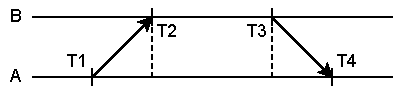
\includegraphics[width=6cm, height=5cm, keepaspectratio]{assets/network-time-protocol.pdf}
\end{center}
Then this will be the procedure:
\begin{enumerate}
	\item $A$ sends a request to $B$ with timestamp $T_1$;
	\item $B$ records $T_2$ from its own clock;
	\item $B$ returns a response containing both $T_1$ and $T_2$;
	\item $A$ records the value $T_4$ from its own clock.
\end{enumerate}
If we assume similar propagation delays then $T_2 - T_1 \approx T_4 - T_3$. This makes client $A$ able to compute the offset between the two clocks as such:
\begin{align*}
	\Theta & = T_3 + \frac{(T_2 - T_1) + (T_4 - T_3)}{2} - T_4 \\[10pt]
	& = T_3 + \frac{\Delta T_{req} + \Delta T_{res}}{2} - T_4
\end{align*}
If $\Theta \neq 0$, then:
\[ C_A := C_A + \Theta \]
Where $C_A$ is \textbf{$A$'s clock} and $\Theta$ is the \textbf{offset between the clocks}.

\subsubsection{Berkeley Algorithm}
While in the NTP (Network Time Protocol) the time server is passive, in \textbf{Berkeley UNIX} the time server polls every machine periodically. Based on the client's response, the time server computes the averages and tells the client to update their timer. The time daemon -- which is the time of the server itself -- is updated manually.
\begin{center}
	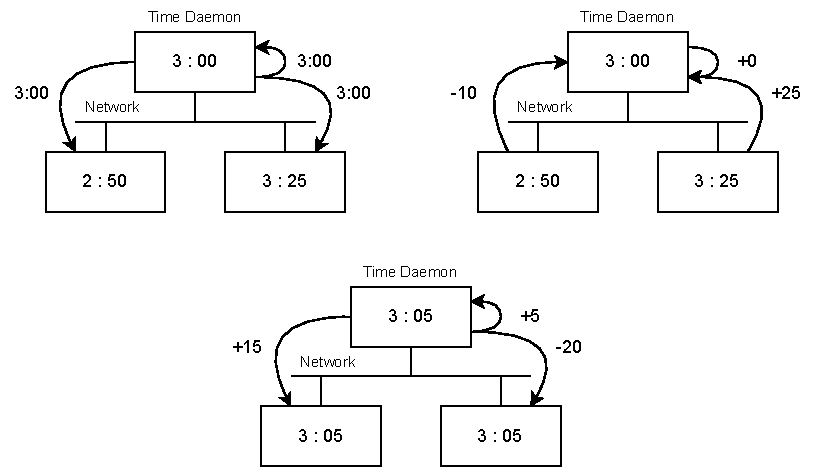
\includegraphics[width=10cm, height=10cm, keepaspectratio]{assets/berkeley-time.pdf}
\end{center}

\subsection{Logical Clocks}
Many applications need to agree on a current time. This time, though, does not need to necessarily match real time. In addition, if two processes don't interact with each other, it's not necessary for their clocks to be synchronised.

\subsubsection{Lamport's Logical Clocks}
Given the \textbf{happened-before} relation depicted by $\rightarrow$, we can say that $a \rightarrow b$ means that event $a$ comes before event $b$. The happens-before relation is \textbf{transitive}, this means that if we have both $a \rightarrow b$ and $b \rightarrow a$, then we can say that events $a$ and $b$ are concurrent. Given the following diagram:
\begin{center}
	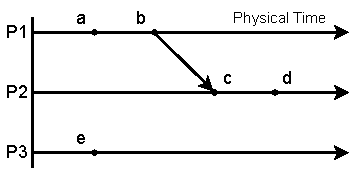
\includegraphics[width=5cm, height=10cm, keepaspectratio]{assets/lamport.pdf}
\end{center}
We can define some other properties:
\begin{itemize}
	\item If $a \rightarrow b$, then $b \nrightarrow a$;
	\item If $a \nrightarrow b$, and $e \nrightarrow a$, then $a \parallel e$;
	\item Even if $b \rightarrow d$, this does not imply causality.
\end{itemize}
Each process $P_i$ keeps a Lamport timestamp $L_i$. A timestamp of event $e$ in $P_i$ is defined as:
\[ T_{P_i} = L_i(e) \]
Where $T$ is the \textbf{timestamp}, $P_i$ is the \textbf{$i$-th process}, $L_i$ is the \textbf{timestamp function}, and $e$ is the \textbf{event's name}.\\ \\
When a process updates its local Lamport clock and wants to transmit its value in a message, then it must follow certain rules, namely:
\begin{itemize}
	\item The Lamport timer $L_i$ must be incremented before each event is issued by the process:
	\[ P_i : L_i = L_i + 1 \]
	\item When process $P_i$ sends a message $m$, the value $t = L_i$ needs to piggyback on message $m$ -- this means that the timestamp must be sent together with the message;
	\item Upon receiving $(m, t)$ -- where $m$ is the \textbf{message} and $t$ is the \textbf{timestamp} -- process $P_j$ will compute:
	\[ L_j = \max(L_j, t) \]
	And applies rule 1 before timestamping the next event -- which will be receive($m$).
\end{itemize}
From the rules above, we can say that
\[ e \rightarrow e' \Rightarrow L(e) < L(e') \]
Where $e$ and $e'$ are the \textbf{two events}, and $L(e)$ and $L(e')$ are the \textbf{Lamport timestamps of those two events}.

\subsubsection{Totally Ordered Logical Clocks}
Since we sometimes need to have a total order of events, Lamport timestamps are not sufficient. The following is an extension of Lamport logical clocks.\\ \\
Let $e_i$ be an event in $P_i$ with timestamp $T_i$, and let $e_j$ be and event in $P_j$ with timestamp $T_j$. We now define two \textbf{global timestamps} as $(Ti, i)$ for $P_i$ and $(T_j, j)$ for $P_j$. The following
\[ (T_i, i) < (T_j, j) \]
Will hold iff either $T_i < T_j$, or $T_i = T_j$ and $i > j$.

\subsubsection{Vector Clocks}
A key property of vector clocks is that:
\[ e \rightarrow e' \Leftrightarrow L(e) < L(e') \]
Given an array of $N$ processes, each process $P_i$ keeps its own vector clock $V_i$. The vector clock is used to timestamp local events. Every process sends the vector's timestamp together with the message to the other process.
\begin{center}
	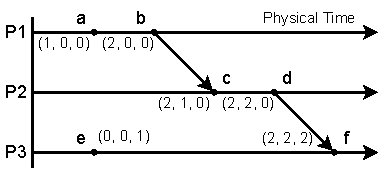
\includegraphics[width=5cm, height=10cm, keepaspectratio]{assets/vector-clocks.pdf}
\end{center}
The vector timestamps in this representation are compared as follows:
\begin{itemize}
	\item $v = v' ~~~~~~~~\text{iff}~V[j] = V'[j] ~~~~~~~~\text{for}~j = 1, 2, 3, \dots, N$
	\item $v \leq v' ~~~~~~~~\text{iff}~V[j] \leq V'[j] ~~~~~~~~\text{for}~j = 1, 2, 3, \dots, N$
	\item $v < v' ~~~~~~~~\text{iff}~V \leq V' ~\text{and}~ V = V'$
\end{itemize}
As with Lamport clocks, also vector clocks have rules for updating the vector. These rules are:
\begin{enumerate}
	\item Initially the vector clock is as follows:
	\[ V_i[j] = 0 ~~~~~~~~\text{for}~j = 1, 2, 3, \dots, N \]
	\item Before process $P_i$ timestamps an event, it sets
	\[ V_i[i] = V_i[i] + 1 \]
	\item Process $P_i$ then needs to include timestamp $t = V_i$ in every message it sends;
	\item When $P_i$ receives a timestamp $t$ in a message, it sets
	\[ V_i[j] = \max(V_i[j], t[j]) ~~~~~~~~\text{for}~j = 1, 2, 3, \dots, N \]
	This operation is called \textbf{merge}.
\end{enumerate}
Where $V_i[j]$ is the \textbf{number of events process $P_i$ has timestamped}, and $V_i[j]$ with $i \neq j$ is the \textbf{number of events at process $P_j$ that have potentially effected $P_i$}.

\subsection{Mutual Exclusion}
Let's assume that we have $N$ processes named $P_i$, that processes do not share variables, that the system is asynchronous, and that there are no process failures. Given these assumptions, we have an application-level interface composed by the following functions:
\begin{itemize}
	\item \verb|enter()|
	\item \verb|resourceAccess()|
	\item \verb|exit()|
\end{itemize}
Some more requirements are needed for the mutual exclusion, namely:
\begin{enumerate}
	\item \textbf{Safety} \\
	At most one process may execute in the critical section at a time.
	\item \textbf{Liveness} \\
	Requests to enter the critical section will eventually succeed. No starvation or deadlocks are allowed.
	\item \textbf{Ordering} \\
	If one request to enter the critical section happened before another, then entry to the critical section is granted in that order.
\end{enumerate}

\subsubsection{Central Server Algorithm}
in this case, a central server handles the requests to enter the critical section by saving each request in a FIFO queue.
\begin{center}
	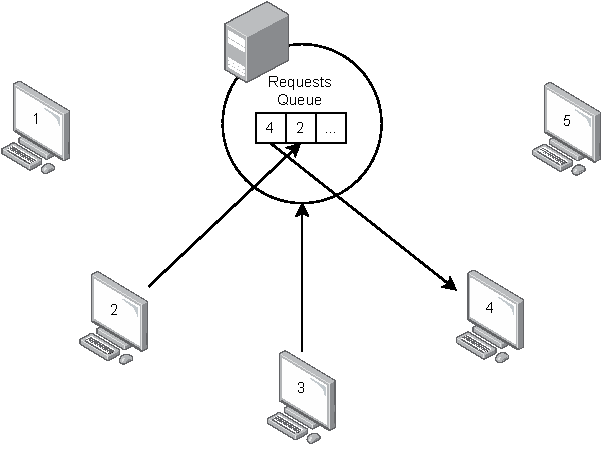
\includegraphics[width=6cm, height=10cm, keepaspectratio]{assets/central-server.pdf}
\end{center}
The actions performed in the image above are the following:
\begin{enumerate}
	\item Process $P_2$ requests the token to access the critical section;
	\item Process $P_3$ releases its token for access to the critical section;
	\item The server grants access to $P_4$ to enter the critical section.
\end{enumerate}
In absence of failures, ME requisites 1 and 2 are respected. ME requisite 3, however, is not respected. Moreover, he central server may become the bottleneck of the whole system in case of heavy loads. The server is also a single-point-of-failure, this means that is the server fails, the whole system shuts down.

\subsubsection{Ring-Based Algorithm}
The processes are now arranged in a logical ring. These processes circulate a token around the ring. As before, the token is needed by the process to access the critical section. If one of the processes has the token, but does not need to enter the critical section, it sends the token to the neighbouring process. This token is passed to the neighbouring process even when the process exits from the critical section.
\begin{center}
	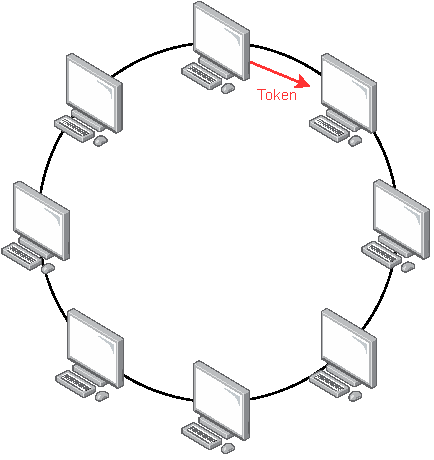
\includegraphics[width=5cm, height=10cm, keepaspectratio]{assets/ring-based.pdf}
\end{center}
ME requisites 1 and 2 are respected, but requisite 3 is not respected. Moreover, bandwidth is consumed even if no process requires access to the critical section.

\subsubsection{Multicast and Logical Clock Algorithm}
The idea of this algorithm is the following:
\begin{enumerate}
	\item The process that requires access to the critical section multicasts a request message to all the other processes;
	\item If a response is received by the process from all of the other processes, then access to the critical section is granted.
\end{enumerate}
We can have two possible scenarios.
\begin{center}
	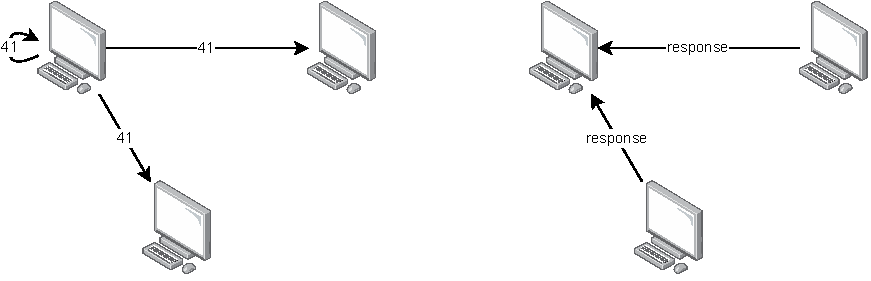
\includegraphics[width=9cm, height=13cm, keepaspectratio]{assets/multicast-1.pdf}
\end{center}
Here, to the process multicasting the request is granted access to the critical section. The reason is that both of the other processes sent a response message back to the requesting process.
\begin{center}
	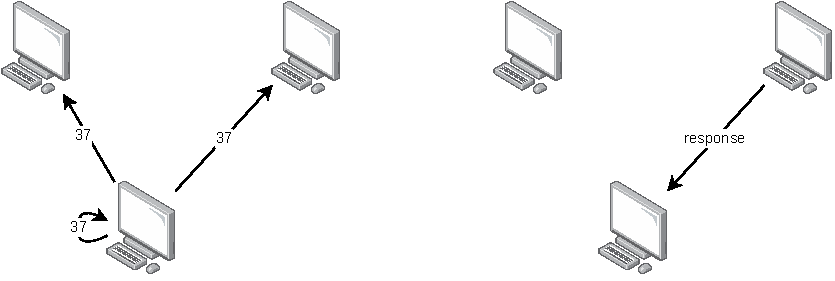
\includegraphics[width=9cm, height=13cm, keepaspectratio]{assets/multicast-2.pdf}
\end{center}
Instead, in this case, the to the process multicasting the request is not granted access to the critical section. The reason is that only one of the other two processes has sent a response message back to the requesting process. \\ \\
This algorithm guarantees ME requisites 1, 2, and 3. Moreover, each process $P_i$ has its own Lamport clock. The messages request entry at time $(T, P_i)$, where $T$ is the \textbf{sender's timestamp}, and $P_i$ is the \textbf{sender's id}. \\ \\
The problem with this algorithm is that every time a process $P_i$ needs access to the critical section, $2(N-1)$ messages need to be exchanged -- for both multicast and replies. Moreover, up to $N - 1$ messages are sent when a process exits the critical section -- since it needs to communicate it to the rest of the processes.

\subsubsection{Maekawa's Voting Algorithm}
Access to the critical section does not need to permission from all of the processes, but from a subset of them is enough -- only if the subsets overlap. \\ \\
This algorithm is very similar to the previous. In this case, though, we need for a sufficient number of votes -- not all. To achieve this, to each process is assigned a voting set $V_i$. \\ \\
ME requirement 1 is respected, but the algorithm is deadlock-prone. By queuing outstanding requests in a happens-before order, then both ME requirements 2 and 3 are also respected. \\ \\
By using this algorithm, we will have $\approx 2 \sqrt{N}$ messages when asking to join the critical section, and $\approx\sqrt{N}$ messages when exiting the critical section.

\subsection{Election Algorithms}
These kind of algorithms are used for choosing a coordinator, which is represented by a single process. The coordinator is like the sever in the server-based mutual exclusion algorithm. \\ \\
Each process $P_i$ has a variable $elected_i$, which is initially set to $\perp$. Moreover, two requirements must always be met. These requirements are:
\begin{enumerate}
	\item \textbf{Safety} \\
	At any point in time
	\[ \forall P_i : elected_i \in \{ \perp, P \} \]
	Where $P$ is a non-crashed process with the largest id;
	\item \textbf{Liveness} \\
	All non-crashed processes $P_i$ will eventually set
	\[ elected_i = P \]
	Where $P$ is a non-crashed process with the largest id.
\end{enumerate}

\subsubsection{Ring-Based Election Algorithm}
Let's suppose that we have an asynchronous system, no failures, processes arranged in a logical ring, and that messages can only circulate in one direction.
\begin{center}
	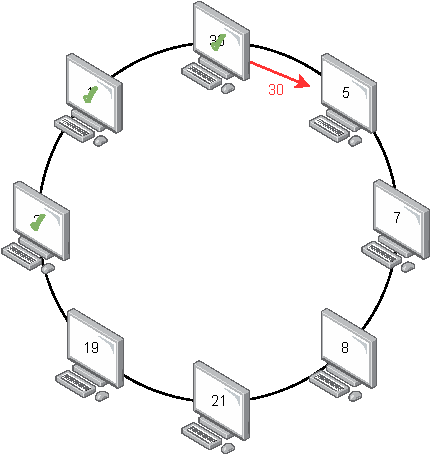
\includegraphics[width=6cm, height=10cm, keepaspectratio]{assets/ring-election.pdf}
\end{center}
The process of election is the following:
\begin{enumerate}
	\item Every process is initially marked as \textbf{non-participant};
	\item To start an election, process $P_i$ makes itself a participant, and places its id onto the message to send to its neighbour;
	\item When $P_j$ receives the message:
	\begin{itemize}
		\item If the id is greater than $P_j$'s id, then the message is forwarded directly to the neighbouring process;
		\item If $P_j$ is not marked as a participant, it is marked as a participant and its id is sent to the neighbouring process.
	\end{itemize}
	\item If $P_i$ receives back its own id after one complete cycle of election, then it is elected as \textbf{leader} and marked as non-participant. Then, it sends  the \textbf{elected} message with its own it to its neighbouring process;
	\item When $P_j$ receives the \textbf{elected} message, it saves the id of the leader and passes the message onwards.
\end{enumerate}
Let's consider the worst-case scenario. Let's say that process $P_i$ starts the election and that the process before it (process $P_j$) is the one with the highest id. In this case we will have the following:
\begin{itemize}
	\item $N-1$ messages needed to reach process $P_j$;
	\item $N$ messages for $P_j$ to announce to the other processes it is now the leader;
	\item $N$ messages for all of the other processes to acknowledge the id of the new leader.
\end{itemize}
A total of $3N-1$ messages are sent for the election process to be complete.

\subsubsection{Bully Algorithm}
In this algorithm, we take into account the fact that a process may crash. However, messages are sent reliably and all processes know every other process' id. Moreover, this is a synchronous system, where:
\begin{itemize}
	\item $T_{trans}$ is the maximum message transmission delay;
	\item $T_{process}$ is the maximum process delay;
	\item $T = 2_{trans} + T_{process}$ is the total elapsed time upper bound.
\end{itemize}
Graphically the process can be represented as follows:
\begin{center}
	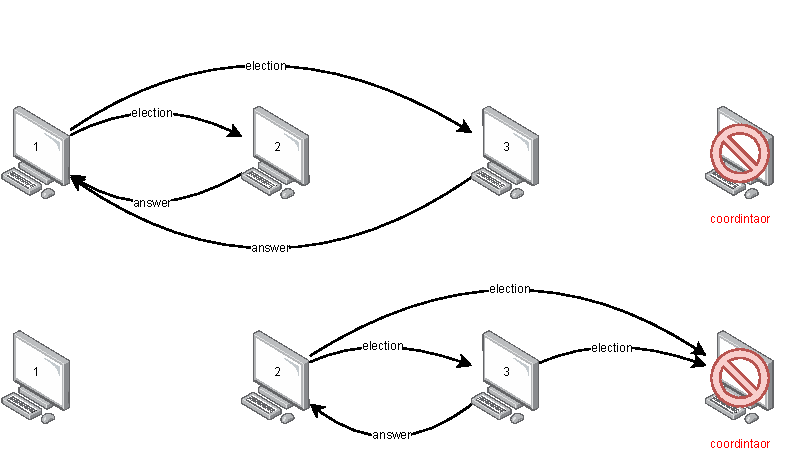
\includegraphics[width=11cm, height=20cm, keepaspectratio]{assets/bully-1.pdf}
\end{center}
\begin{center}
	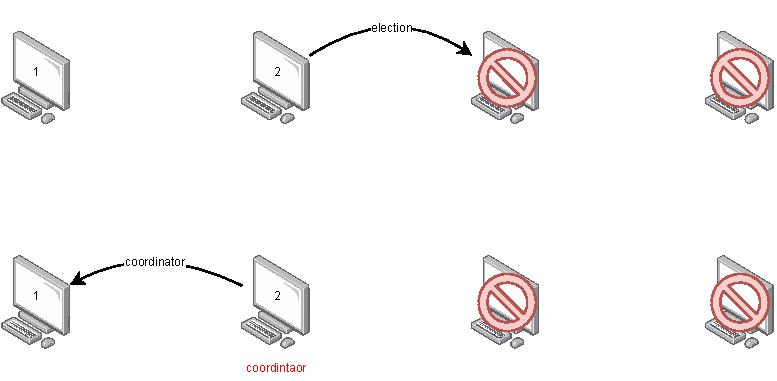
\includegraphics[width=11cm, height=20cm, keepaspectratio]{assets/bully-2.pdf}
\end{center}
The steps performed by the algorithm are the following:
\begin{enumerate}
	\item Let $P_1$ suspect the crash of the current leader: process $P_4$;
	\item If $P_1$ has the highest id, then
	\begin{itemize}
		\item Send a \textbf{coordinator} message to all other processes with lower id  to elect itself as the new leader;
		\item Otherwise, $P_1$ sends an \textbf{election} message to all the processes with higher id, and awaits for an \textbf{answer} message.
	\end{itemize}
	\item If no \textbf{answer} message arrives within the predefined time $T$, then
	\begin{itemize}
		\item $P_2$ considers itself the leader and sends a \textbf{coordinator} message to all processes with lower id;
		\item Otherwise, $P_2$ awaits another period $T$ for a \textbf{coordinator} message. If none arrives, then $P_2$ will start a new election.
	\end{itemize}
	\item If $P_1$ receives a \textbf{coordinator} message, it sets
	\[ selected_1 = P_2 \]
	\item If $P_1$ receives an \textbf{election} message, it will answer with an \textbf{answer} message and starts a new election -- if one hasn't already been started.
\end{enumerate}
In the best-case scenario, $N-1$ messages will be exchanged. In the worst-case scenario, $N^2$ messages will be exchanged.

\section{Replication and Consistency}
\textbf{Replication} guarantees several different things:
\begin{itemize}
	\item \textbf{Reliability} \\
	It protects against both failure and corrupted data;
	\item \textbf{Performance} \\
	It helps in scaling up numbers of clients and geographical area. By increasing the number of clients, it follows an increase in the number of processes needing access to data.
\end{itemize}
The main problem with replication is that multiple copies may lead to consistency issues. For this reason, we should modify the copies or the original with caution. \\ \\
The solution to consistency problems could be solved by \textbf{loose consistency}. This means that global synchronisation is avoided -- because too expensive, and that replica states may diverge.

\subsection{Data-Centric Consistency Models}
\subsubsection{Data Store}
In these kinds of models, we have a \textbf{distributed data store} on which read and write operations are performed.
\begin{center}
	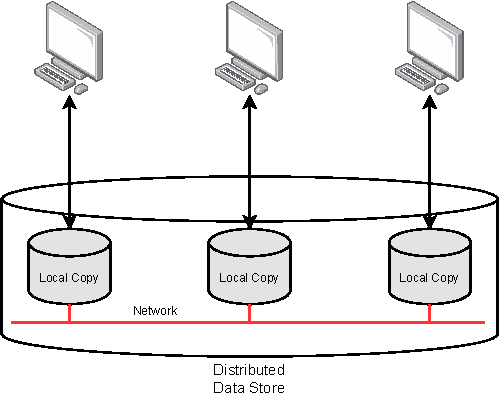
\includegraphics[width=6cm, height=10cm, keepaspectratio]{assets/data-store.pdf}
\end{center}

\subsubsection{Consistency Model}
A contract exists between the processes and the data store. If this contract -- i.e. set of rules -- is respected by the processes, then the store will work correctly.
\begin{center}
	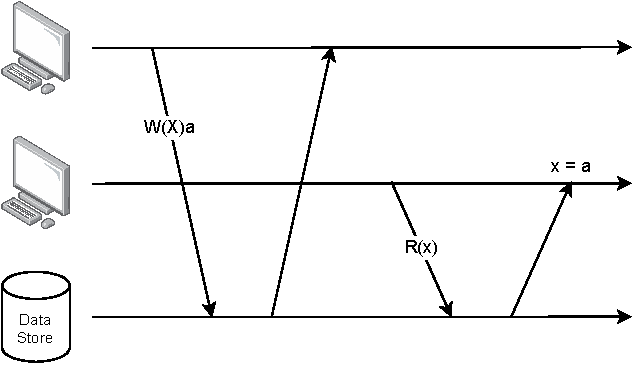
\includegraphics[width=7cm, height=10cm, keepaspectratio]{assets/consistency.pdf}
\end{center}

\subsubsection{Sequential Consistency}
This concept was first introduced by Lamport. Read and write operations are allowed, and the variables are all initially set to NIL. \\ \\
A data store is said to be \textbf{sequentially consistent} when the result of any execution is the same as if the read and write operations were executed in some sequential order. Moreover, the operations of each individual process appear in the program the same way as they appear in the sequence. In this case, time is not taken into consideration.
\begin{center}
	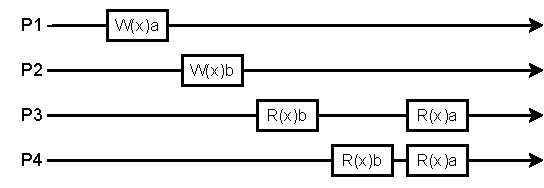
\includegraphics[width=7cm, height=10cm, keepaspectratio]{assets/sequential-consistency.pdf}
\end{center}

\subsubsection{Causal Consistency}
Writes that are potentially causally related, must be seen by all the processes in the same order. Concurrent writes may be seen in a different order on different by different machines.
\begin{center}
	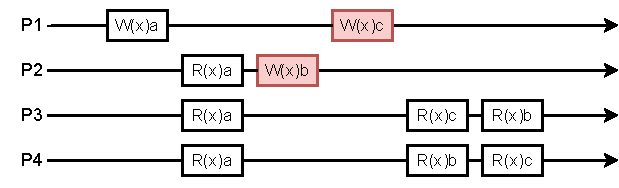
\includegraphics[width=8cm, height=10cm, keepaspectratio]{assets/causal-consistency.pdf}
\end{center}
In the case above, write operations $W_{P_2}(x)b$ and $W_{P_1}(x)c$ are concurrent. Although being concurrent, this execution is causally consistent.

\subsubsection{Entry Consistency}
Sequential and causal consistency were initially developed for shared-memory multiprocessor systems. These paradigms do not work well in the case of distributed systems. 
\begin{center}
	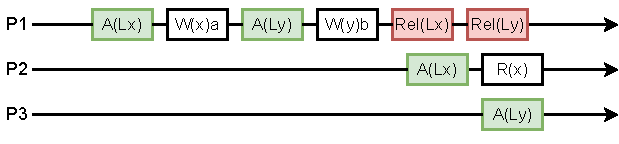
\includegraphics[width=9cm, height=10cm, keepaspectratio]{assets/entry-consistency.pdf}
\end{center}
Processes, before being able to modify shared data, must acquire a lock. This lock will then be released when the data has been successfully modified. A lock is associated with every data item.

\subsection{Client-Consistency Models}
\subsubsection{Eventual Consistency}
In the case of eventual consistency, we have a special class of distributed data stores. Here, the workload is mostly composed of reads and few -- if any -- writes. Data stores use a \textbf{weak consistency} policy. \\ \\
These kind of distributed and replicated databases tolerate a high degree of inconsistency. In the absence of updates, all replicas converge to the same state. This is known as \textbf{eventual consistency}. \\ \\
Some issues with this approach are:
\begin{itemize}
	\item Unreliable network connectivity and poor performance
	\item Processes may connect to different copies and submit read and write commands.
\end{itemize}
In the following sections, four different types of consistencies will be explained in detail.

\subsubsection{Monotonic Reads}
A data store is said to provide monotonic-read consistency is the following holds:
\begin{changemargin}{0.4cm}{0cm} 
If a process reads the value of data item $x$, any successive read operation on $x$ by that process will always return that same value or a more recent value.
\end{changemargin}
An example of monotonic-read consistent data store is the following:
\begin{center}
	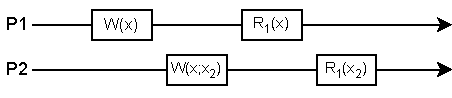
\includegraphics[width=6cm, height=10cm, keepaspectratio]{assets/monotonic-reads.pdf}
\end{center}

\subsubsection{Monotonic Writes}
A data store is said to be monotonic-write consistent if the following condition holds:
\begin{changemargin}{0.4cm}{0cm} 
A write operation by a process on a data item $x$ is completed before any successive write operation on $x$ by the same process -- similarly to FIFO ordering.
\end{changemargin}
An example of monotonic-write consistent data store is the following:
\begin{center}
	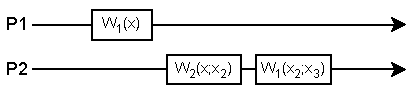
\includegraphics[width=5.5cm, height=10cm, keepaspectratio]{assets/monotonic-writes.pdf}
\end{center}

\subsubsection{Read your Writes}
A data store is said to provide read-your-writes consistency if the following condition holds:
\begin{changemargin}{0.4cm}{0cm} 
The effect of a write operation by a process on data item $x$ will always be seen by successive read operations on $x$ mad by the same process.
\end{changemargin}
An example of a data store with read-your-writes consistency is the following:
\begin{center}
	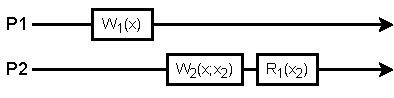
\includegraphics[width=5.5cm, height=10cm, keepaspectratio]{assets/read-your-writes.pdf}
\end{center}

\subsubsection{Writes follow Reads}
A data store is said to provide writes-follow-reads consistency if the following condition holds:
\begin{changemargin}{0.4cm}{0cm} 
A write operation on data item $x$ following a previous read operation on $x$ -- by the same process -- is guaranteed to take place. Moreover, it will take place on the same or more recent value of $x$ that was read.
\end{changemargin}
An example of a data store that provides writes-follow-reads consistency is the following:
\begin{center}
	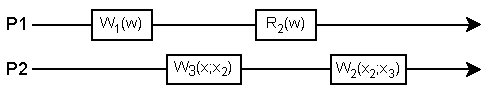
\includegraphics[width=7cm, height=10cm, keepaspectratio]{assets/writes-follow-reads.pdf}
\end{center}

\subsection{Replica Management}
The objectives of replica management are mainly two:
\begin{itemize}
	\item Find the best location for a server that can host part of the data;
	\item Find the best servers for content placement.
\end{itemize}

\subsection{Replica Server Placement}
The placement of the replica represents an optimisation problem. As such, we need heuristics to solve it. We need to find the best $k$ locations out of the $N$ possible locations -- where $k < N$.

\subsection{Content Distribution}
First we need to decide what is there to propagate. Several options are possible:
\begin{itemize}
	\item Propagate only the notification of an update;
	\item Transfer data from one copy to the other;
	\item Propagate the update operation to the other copies.
\end{itemize}
There are \textbf{push} and \textbf{pull} protocols to deal with update propagation.
\begin{itemize}
	\item \textbf{Push-Based Model} \\
	Updates the propagated data without replicas asking for updates. This type of protocol is usually used to obtain a high degree of consistency.
	\item \textbf{Pull-Based Model} \\
	Here the client is the one who asks for updates. This type of protocol is usually used to update caches.
\end{itemize}
There are also two modes of updates communication. These are:
\begin{itemize}
	\item \textbf{Unicasting} \\
	To update $N$ servers we need to send $N$ messages. This communication mode is more suitable for pull-based propagation.
	\item \textbf{Multicasting} \\
	The underlying network will take care of propagating the updates to the clients. This method is very effective when the replicas are in the same LAN (Local Area Network). This mode of communication is more suitable for push-based propagation.
\end{itemize}

\subsection{Consistency Protocols}
\subsubsection{Primary-Based Protocols}
Each data item $x$ in the data store has a \textbf{primary} -- i.e. an original copy. This primary is responsible for coordinating write operations on $x$. There are two main classes of primary-based protocols:
\begin{itemize}
	\item \textbf{Remote-Write Protocols} \\
	This is a primary backup. The write operations are forwarded to a fixed single server.
	\item \textbf{Local-Write Protocols} \\
	The primary migrates between servers. This is a primary-backup protocol, in which the primary migrates to the process that wants to perform the update.
\end{itemize}

\subsection{Replicated-Write Protocols}
Write operations are executed at multiple replicas, not only at the primary. To perform these multiple write operations, we can use one of the following protocols:
\begin{itemize}
	\item \textbf{Active Replication} \\
	In this case, each replica receives and executes all commands. These commands need to be executed in the same order for all replicas. Lamport's total order protocol- or sequencer-based mechanism is used to totally order the commands.
	\item \textbf{Quorum-Based Protocol} \\
	The clients request and acquire permission of multiple servers before being able to read and write to a replicated data item. Read quorum $N_R$ and write quorum $N_W$ are:
	\[ N_R + N_W > N \]
	\[ N_W > \frac{N}{2} \]
\end{itemize}

\end{document}



































